\section{Systematic uncertainties}
\label{sec:systematics}

Besides the systematics related to the background estimation techniques discussed in Sec.~\ref{sec:background_estimations} we following the ICHEP recommendations~\cite{twiki:sys} for signal systematics and the POG recommended experimental uncertainties.

%%% Uncorrelated point by point MC statistical uncertainty

Specifically, the jet energy scale (JES) is varied within uncertainty~\cite{Chatrchyan:2011ds} as a function of jet \pt and $\eta$, and
these changes are propagated to all observables, including \ETmiss. The \ETmiss observable is moreover subject to uncertainties from the 
unclustered energy which is varied within uncertainties.

The simulated efficiencies for the identification of b-quark jets and for the misidentification of c-quark,
light-quark or gluon jets need to be corrected for with scale factors and their respective uncertainties~\cite{CMS-PAS-BTV-15-001} are evaluated using method 1a~\cite{twiki:btagSF}.

Uncertainties for the efficiency of lepton reconstruction and identification according to the ICHEP data set are handled in the same way. We consider
lepton-ID efficiencies (electrons and muons separately) that were derived for our particular lepton definition. Moreover, we correct the simulation based
on studies of the HIP effect (heavily ionizing particle) that accounts for a dynamic inefficiency of the silicon strip tracker and hence a reduction in tracking efficiency
as a function of instantaneous luminosity. 

To adjust the simulated PU activity to data, we perform a rewighting based on a total inelastic crossection of 69.2~mb and apply a 5\% uncertainty that we propagate to the reweighting histogram..
The luminosity is measured with the pixel cluster counting method, and the absolute luminosity scale calibration is derived from
an analysis of Van der Meer scans performed in May 2016, resulting in an uncertainty of 6.2\%~\cite{LUMI2016}

Trigger efficiencies are applied as described in Sec.\ref{sec:trigger} and the corresponding bin-by-bin uncertainties are applied as systematics in a correlated way.
Uncertainties on the lepton scale factors following the POG prescriptions~\citep{twiki:eSFsys}.
When a background or signal yield is taken from a simulated sample, the statistical uncertainties are taken into account.
These uncertainties discussed so far, apply to both the background prediction and the signal yield.

Specifically for the backgrounds, the \pt distribution of the top quarks in \ttbar events have found to be softer in 8 \TeV data compared to the prediction by various simulations. 
Based on the NNLO prediction, which gives a reasonable description of the \pt spectrum in data,
a reweighting function has been introduced to alter the shape according to $\sqrt{w(t)\cdot w(\overline{t})}$ where
\begin{equation}
w(\pt) = e^{0.148-0.00129\pt}.
\end{equation}
The reweighting is applied such that it preserves the normalization of the sample, and the difference relative to the results obtained with the unweighted sample is assigned as a systematic uncertainty.

For the signals, an uncertainty on initial-state radiation (ISR) is applied, based on the number of jets which are not matched to simulated particles descending from top quarks, W,Z or Higgs bosons or SUSY particles. The event is reweighted based on the distribution of this observables but correcting for the total change in the crosssection of the respective mass point.
The factorization and renormalization scale are each changed by a factor of 0.5 and 2 and the envelope of variations on the predicted signal yield is assigned as systematic; anti-correlated variations
are not considered.
Finally, uncertainties in the signal cross section are also taken into account.

\subsection{Kinematic distributions in the pre-selection}
\label{sec:preselectionplots}
Figures~\ref{fig:jetsSys} and \ref{fig:mt2llSys} show the distributions of number of jets, medium $b$-tags and \mtll, \mtbb and \mtlblb variables including uncertainty bands from the JEC, \ETmiss uncertainties, top \pt and PU reweighting systematics.
Figure~\ref{fig:mt2bbSys} shows \mtbb and \mtlblb after selecting events with $\mtll > 100$ GeV, where scale factors for $t\bar{t}$, DY, diboson and $t\bar{t}Z$ backgrounds are applied, and their shape uncertainties
are added to the uncertainty band.

\begin{figure}
\centering
\subfloat[]{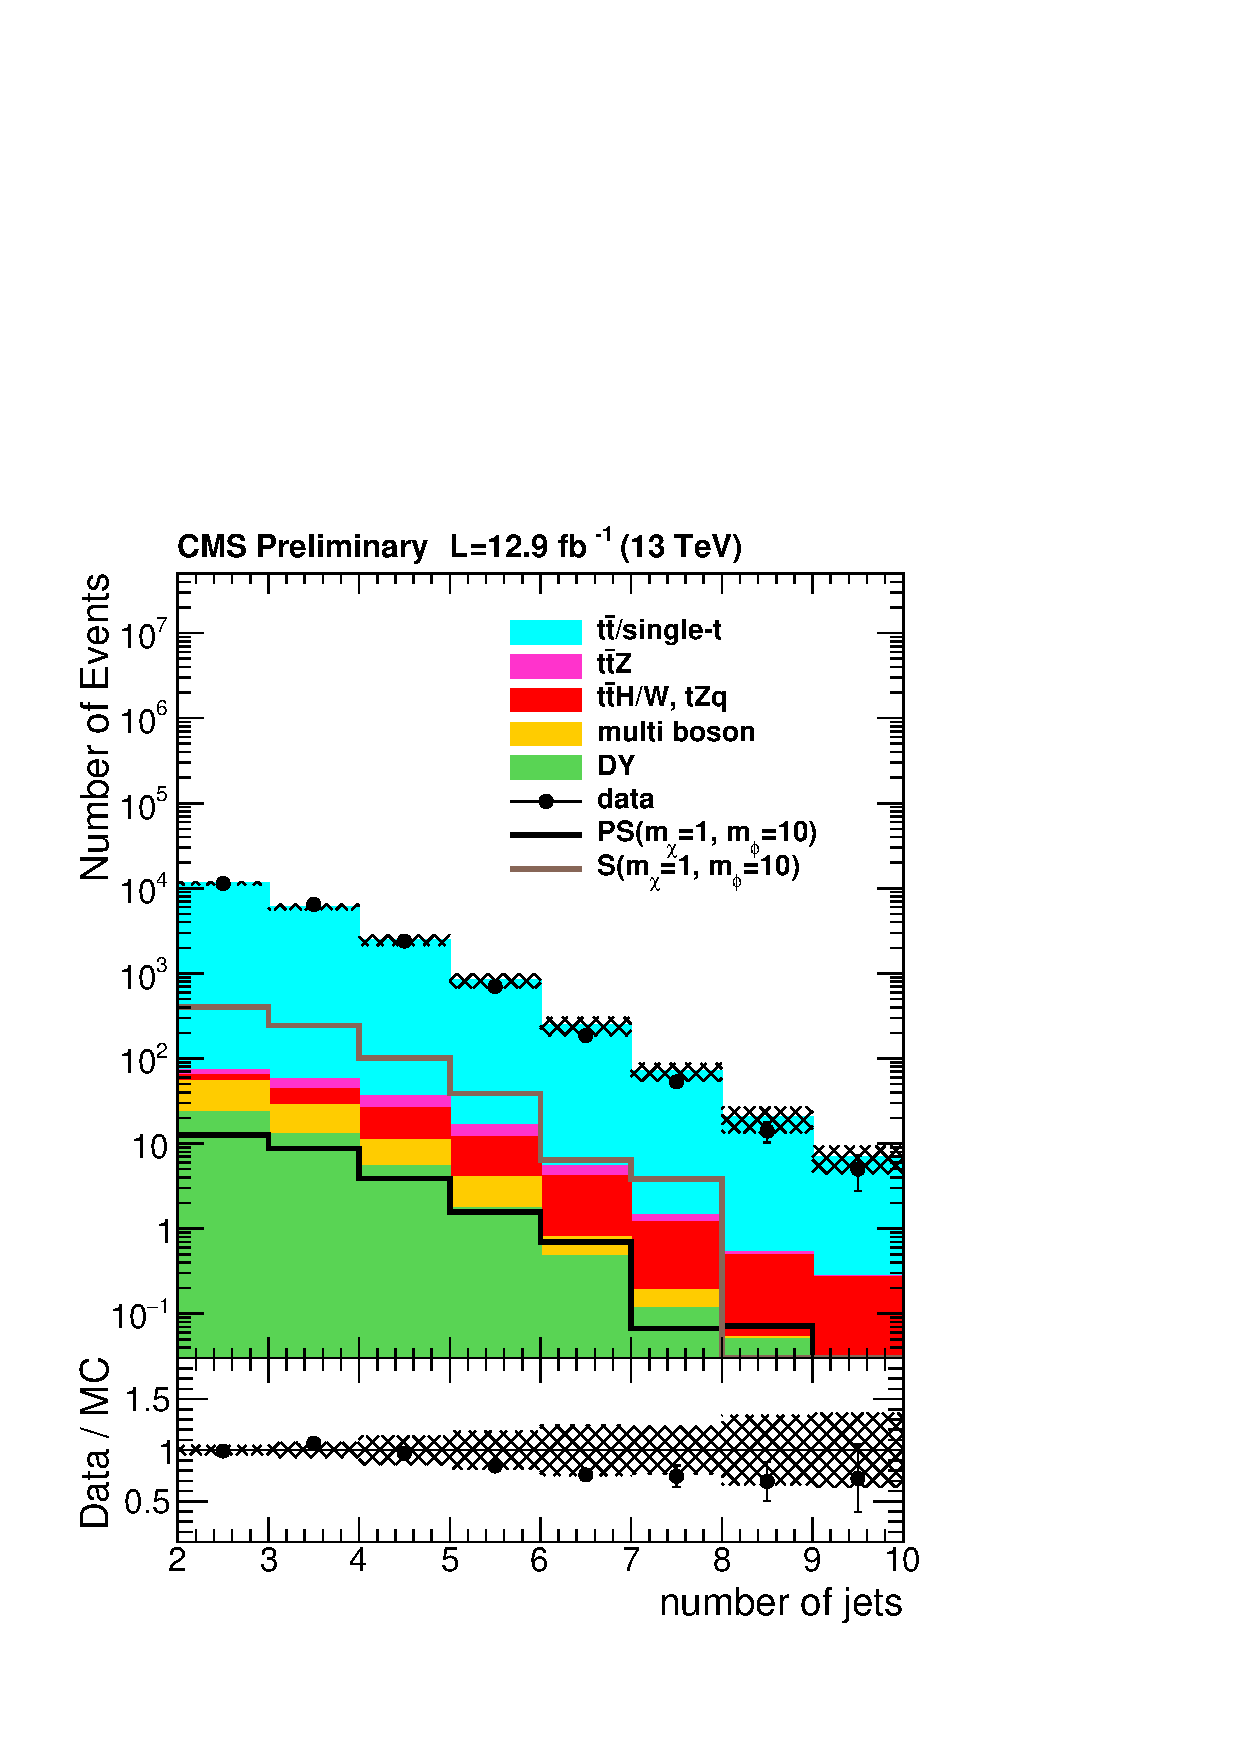
\includegraphics[width=0.45\textwidth]{figures/systematicPlots/all_log_scaled/njet2-btagM-multiIsoWP-looseLeptonVeto-mll20-met80-metSig5-dPhiJet0-dPhiJet1/njets_normalizeBinWidth.pdf}}
\subfloat[]{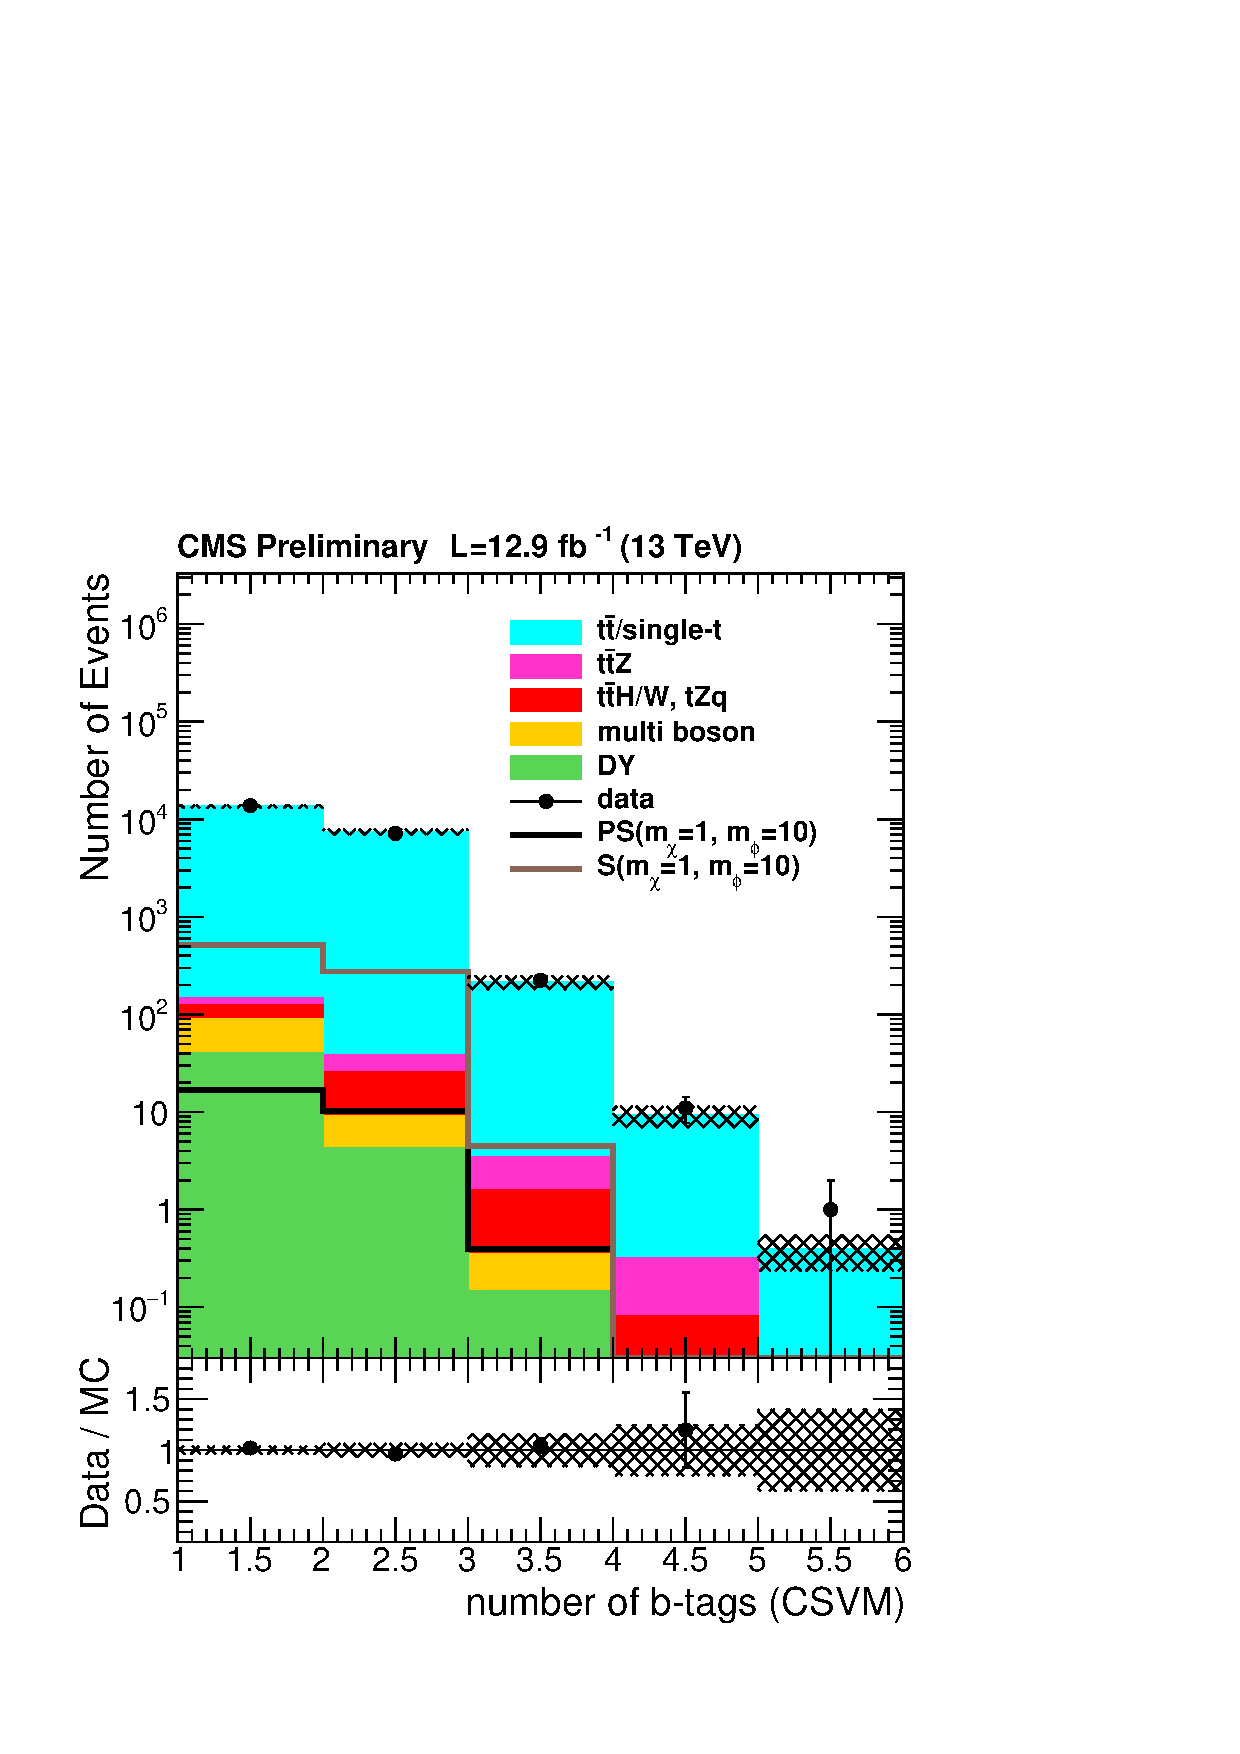
\includegraphics[width=0.45\textwidth]{figures/systematicPlots/all_log_scaled/njet2-btagM-multiIsoWP-looseLeptonVeto-mll20-met80-metSig5-dPhiJet0-dPhiJet1/nbtags_normalizeBinWidth.pdf}}
\caption{Number of jets and medium $b$-tags}
\label{fig:jetsSys}
\end{figure}


\begin{figure}
\centering
\subfloat[]{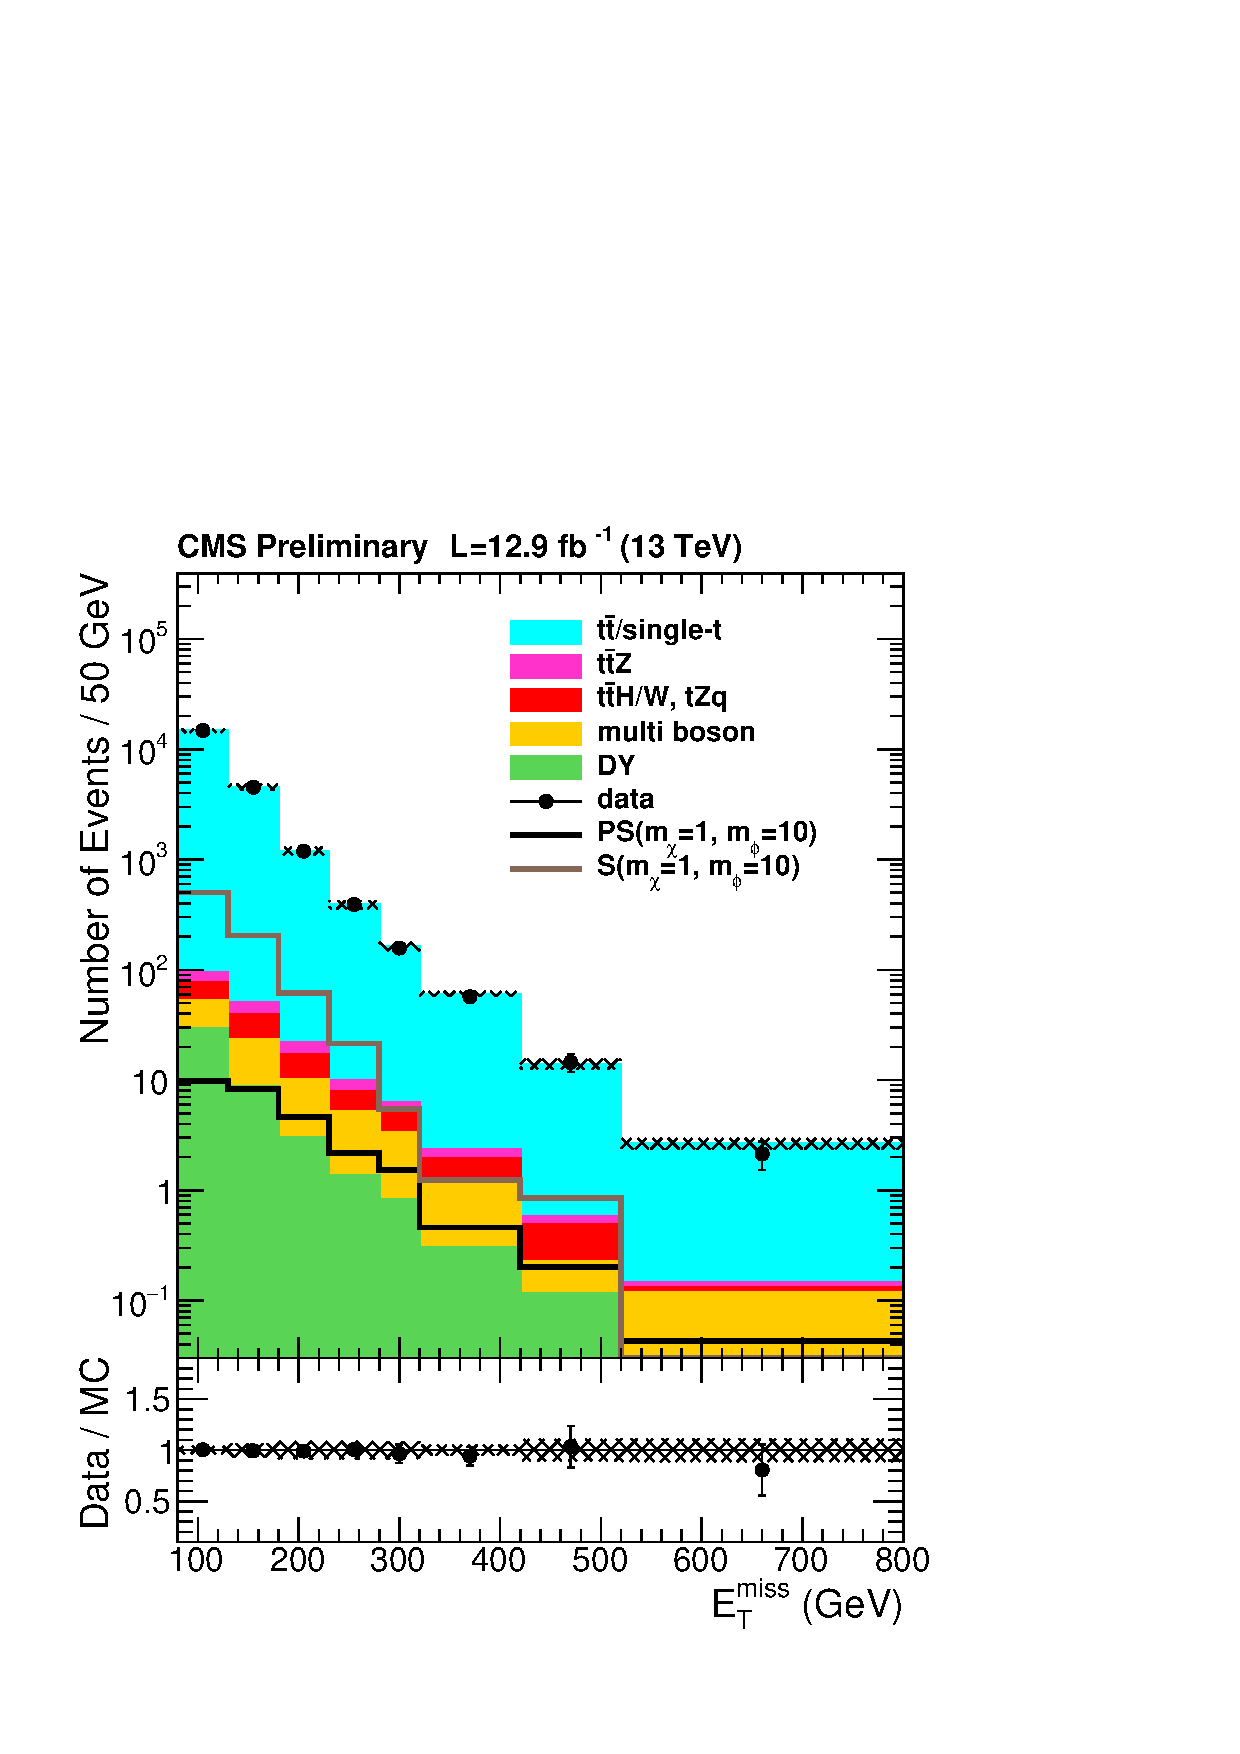
\includegraphics[width=0.45\textwidth]{figures/systematicPlots/all_log_scaled/njet2-btagM-multiIsoWP-looseLeptonVeto-mll20-met80-metSig5-dPhiJet0-dPhiJet1/met_pt_normalizeBinWidth.pdf}}
\subfloat[]{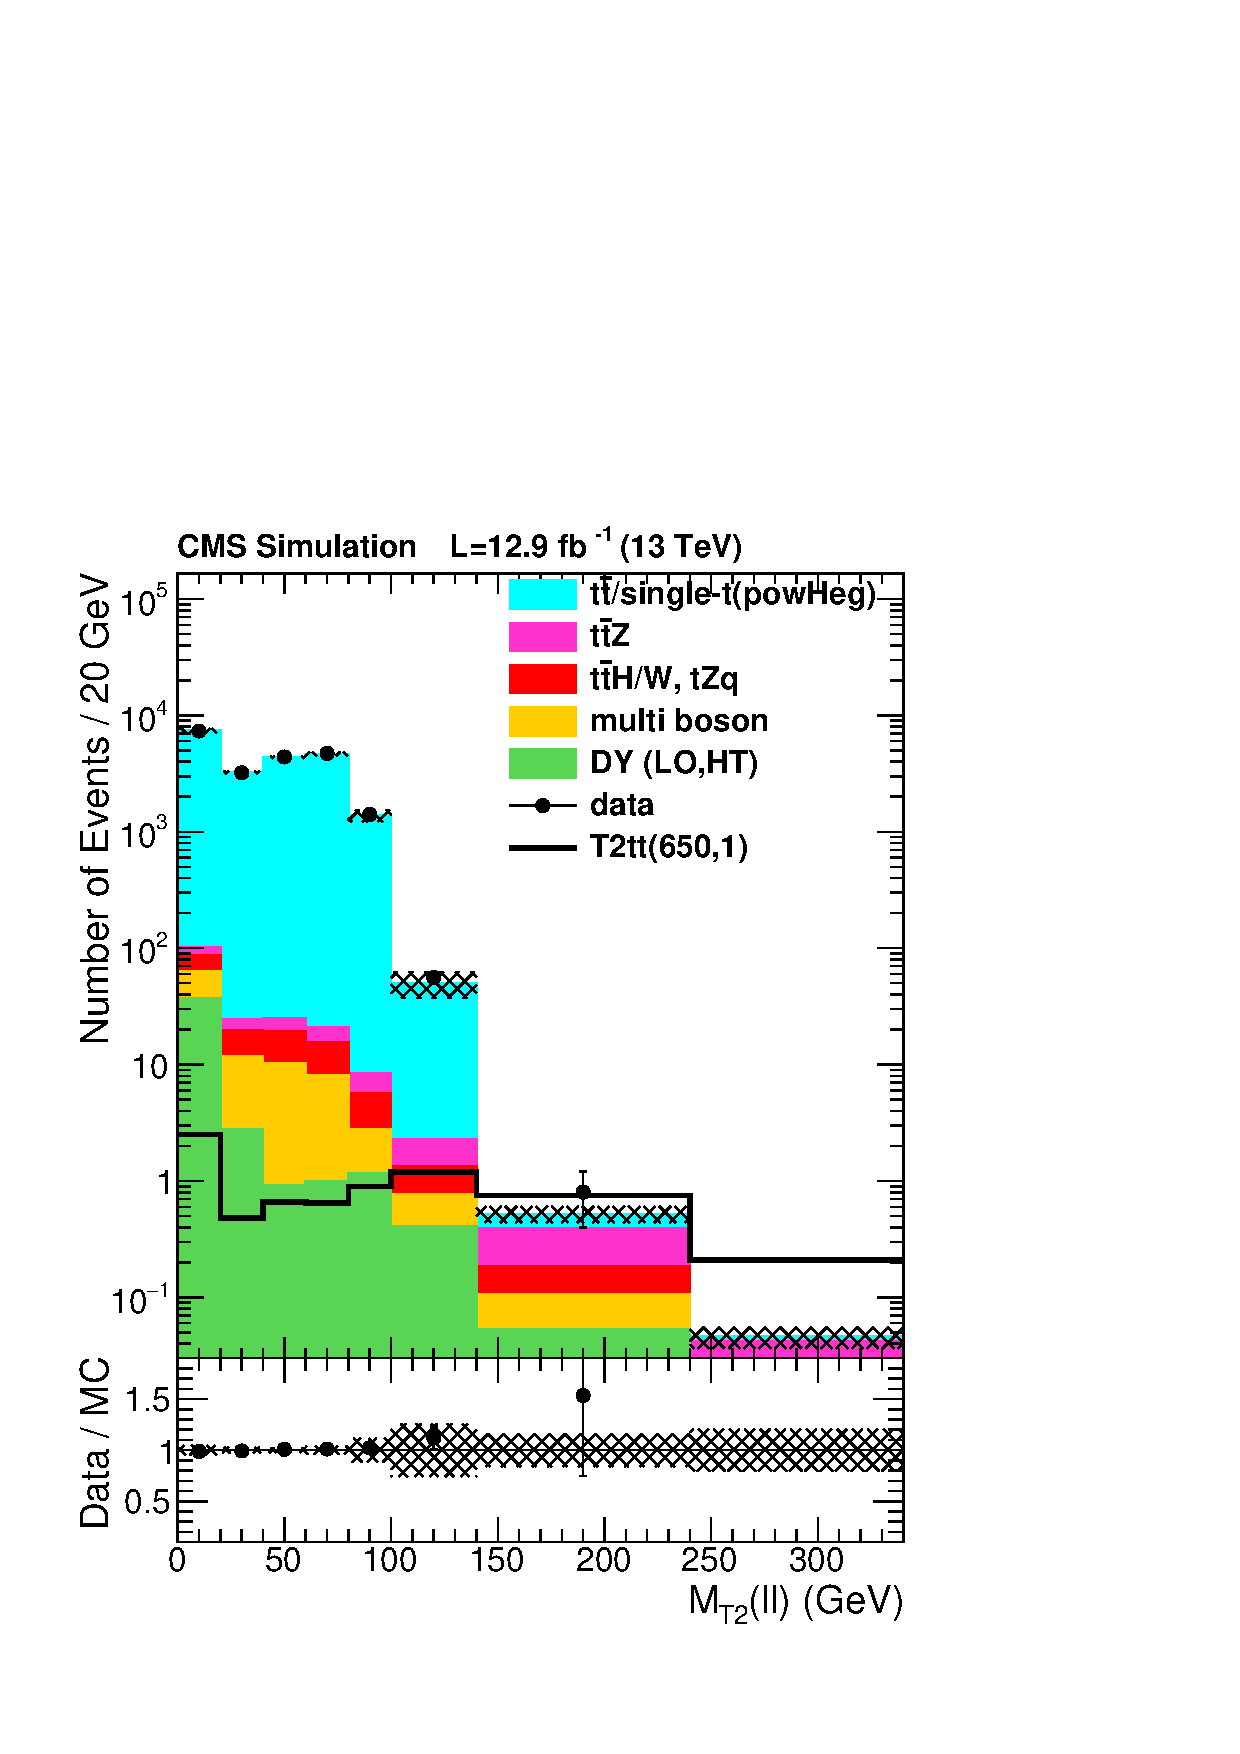
\includegraphics[width=0.45\textwidth]{figures/systematicPlots/all_log_scaled/njet2-btagM-multiIsoWP-looseLeptonVeto-mll20-met80-metSig5-dPhiJet0-dPhiJet1/dl_mt2ll_normalizeBinWidth.pdf}} \\
\caption{Distributions of \ETslash and \mtll after pre-selection.}
\label{fig:mt2llSys}
\end{figure}

\begin{figure}
\centering
\subfloat[]{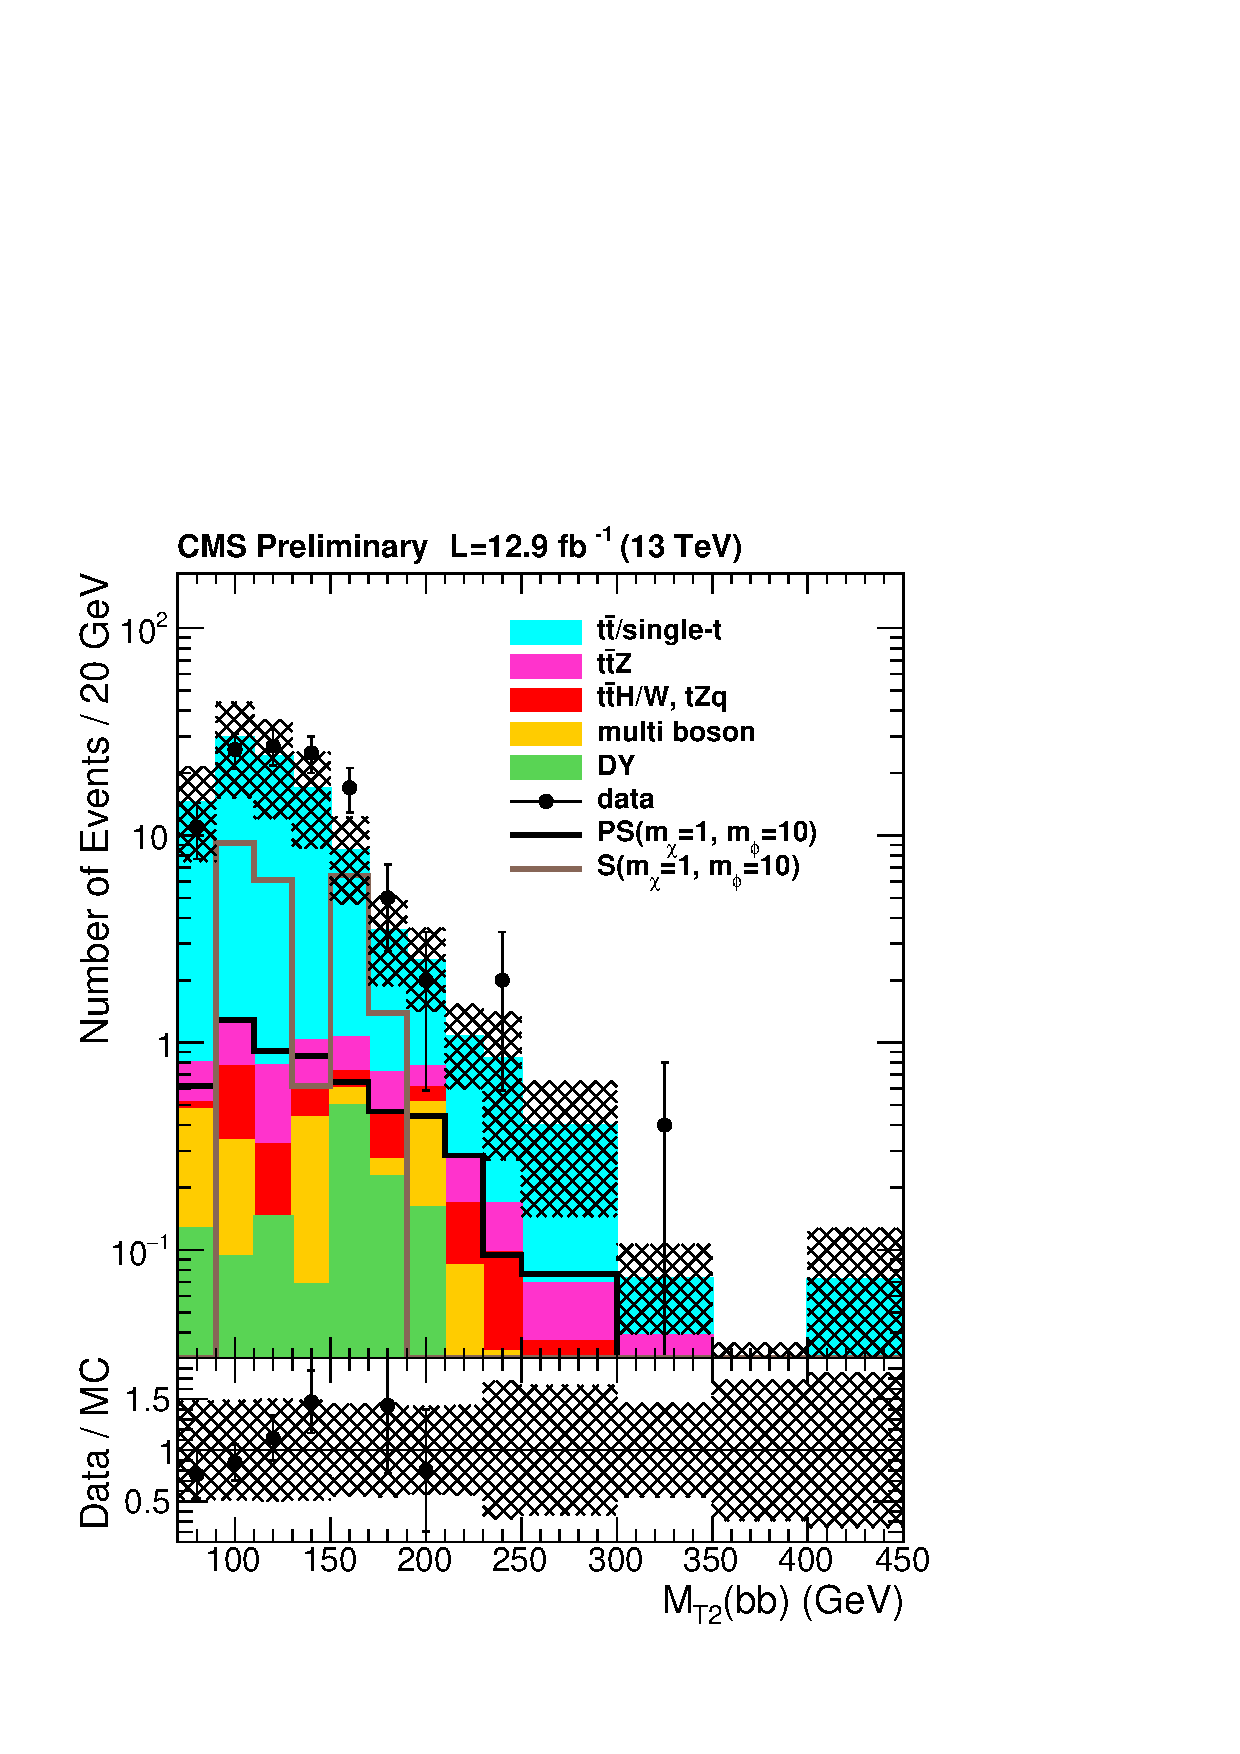
\includegraphics[width=0.45\textwidth]{figures/systematicPlots/all_log_scaled/njet2-btagM-multiIsoWP-looseLeptonVeto-mll20-met80-metSig5-dPhiJet0-dPhiJet1-mt2ll100/dl_mt2bb_normalizeBinWidth.pdf}}
\subfloat[]{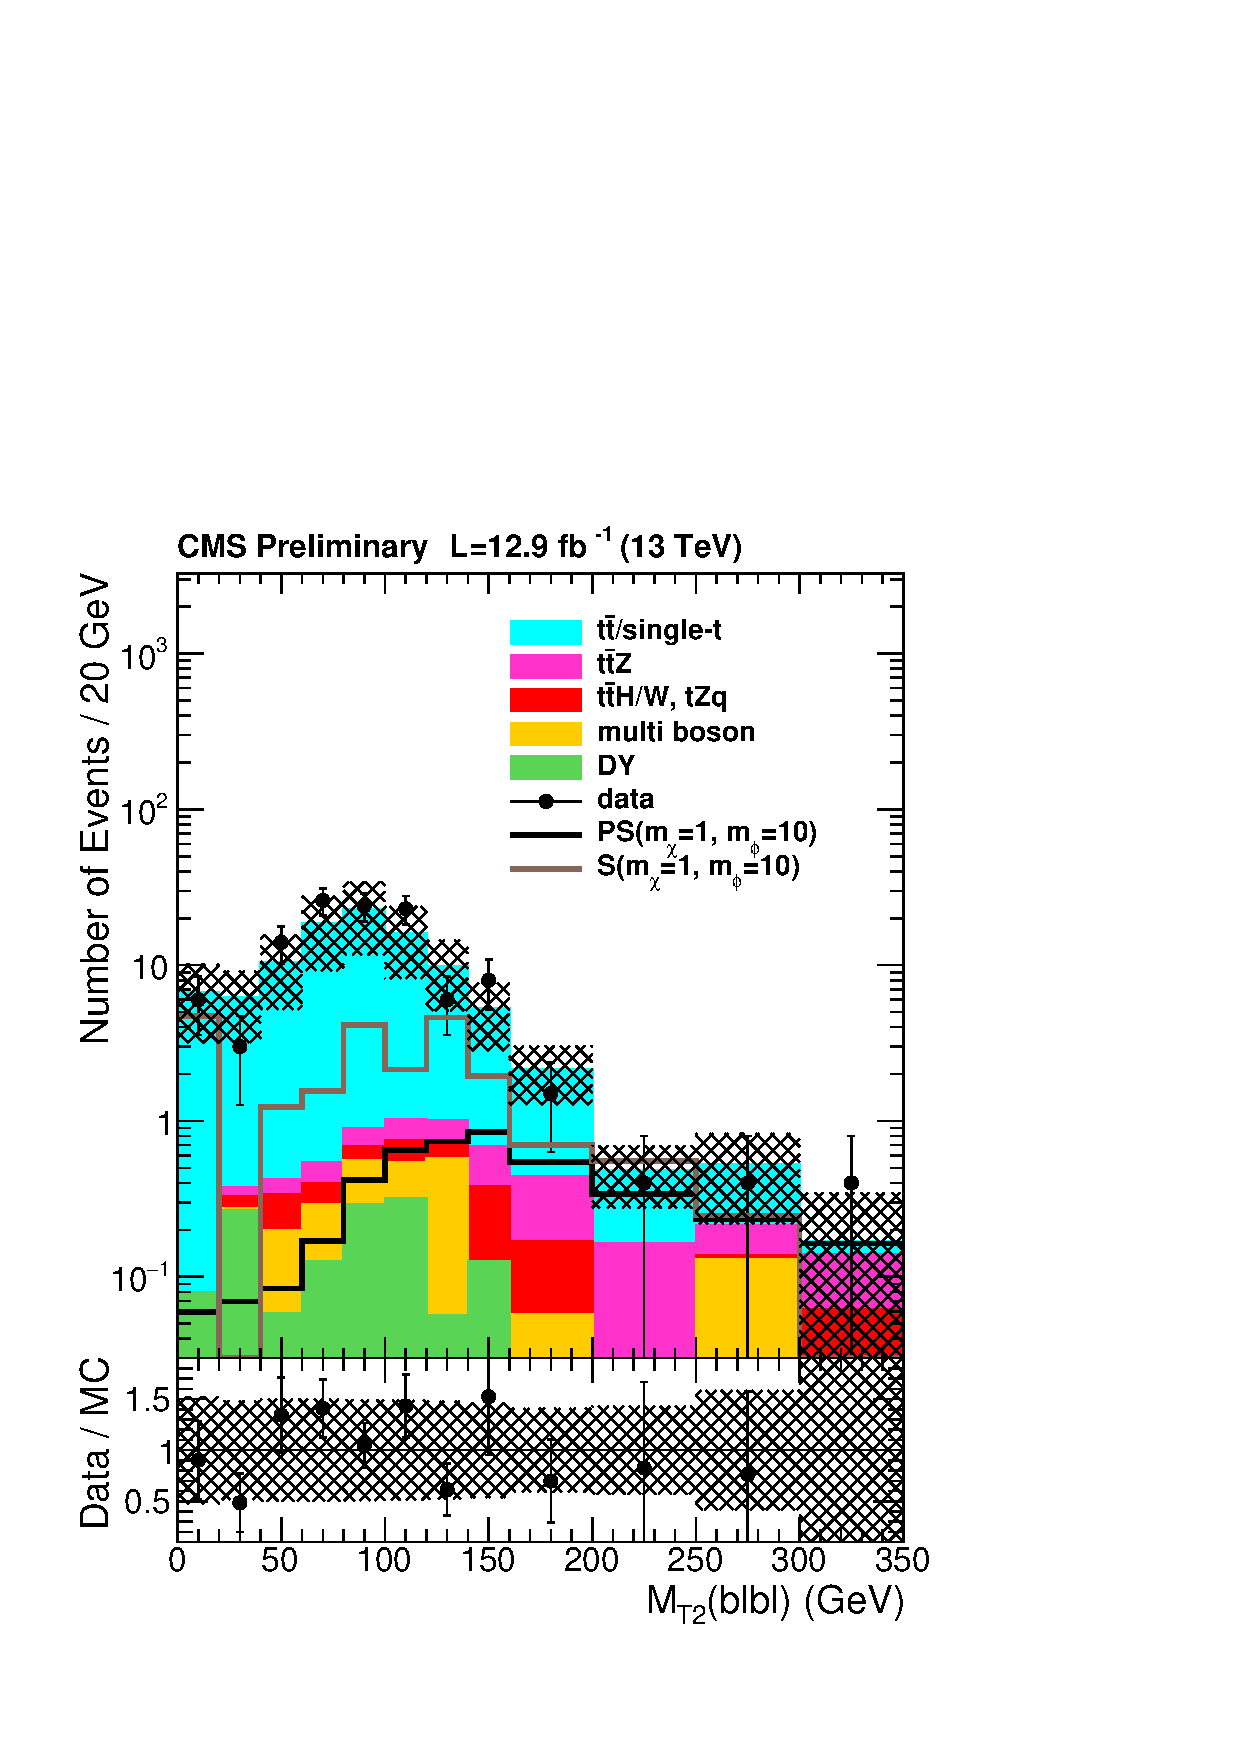
\includegraphics[width=0.45\textwidth]{figures/systematicPlots/all_log_scaled/njet2-btagM-multiIsoWP-looseLeptonVeto-mll20-met80-metSig5-dPhiJet0-dPhiJet1-mt2ll100/dl_mt2blbl_normalizeBinWidth.pdf}}
\caption{Distributions of \mtbb and \mtlblb after pre-selection and $\mtll > 100$ GeV. Scale factors are applied for the $t\bar{t}$, DY, diboson and $t\bar{t}Z$ backgrounds.}
\label{fig:mt2bbSys}
\end{figure}

\begin{table}
\centering
\begin{tabular}{l|c} 
  systematic & min-max of signal regions (\%) \\ 
  \hline 
MC statistics & 4  - 40  \\ 
pile-up & $<$ 14  \\ 
JEC & $<$ 36  \\ 
top-\pt & $<$ 3  \\ 
trigger & $<$ 1  \\ 
lepton SF & $<$ 3  \\ 
b-tag SF-b & $<$ 4  \\ 
b-tag SF-l & $<$ 5  \\ 
top background & $<$ 50  \\ 
$t\bar{t}Z$ background & $<$ 12  \\ 
multiboson background & $<$ 10  \\ 
$t\bar{t}X$ (excl. $t\bar{t}Z$) background & $<$ 8  \\ 
DY background & $<$ 12  \\ 
\end{tabular} 

\caption{Minimal and maximal relative errors for the systematics over all signal regions (all channels combined). Numbers are given relative to the total background contribution per signal region.}
\end{table}
